% Chapter 8: Seminar - Modern Extensions
% ARFIMA, Machine Learning, LSTM
% Bachelor program, Bucharest University of Economic Studies

\documentclass[9pt, aspectratio=169, t]{beamer}

% Ensure content fits on slides
\setbeamersize{text margin left=8mm, text margin right=8mm}

%=============================================================================
% THEME AND STYLE CONFIGURATION
%=============================================================================
\usetheme{default}
% Using default theme for clean header/footer control

% Color Palette (matching Redispatch PDF)
\definecolor{MainBlue}{RGB}{26, 58, 110}
\definecolor{AccentBlue}{RGB}{26, 58, 110}
\definecolor{IDAred}{RGB}{205, 0, 0}
\definecolor{DarkGray}{RGB}{51, 51, 51}
\definecolor{MediumGray}{RGB}{128, 128, 128}
\definecolor{LightGray}{RGB}{248, 248, 248}
\definecolor{VeryLightGray}{RGB}{235, 235, 235}
\definecolor{KeynoteGray}{RGB}{218, 218, 218}
\definecolor{SectionGray}{RGB}{120, 120, 120}
\definecolor{FooterGray}{RGB}{100, 100, 100}
\definecolor{Crimson}{RGB}{220, 53, 69}
\definecolor{Forest}{RGB}{46, 125, 50}
\definecolor{Amber}{RGB}{181, 133, 63}
\definecolor{Orange}{RGB}{230, 126, 34}
\definecolor{Purple}{RGB}{142, 68, 173}

% Gradient background (exact Keynote 315° gradient: white to RGB 218,218,218)
\setbeamertemplate{background}{%
    \begin{tikzpicture}[remember picture, overlay]
        \shade[shading=axis, shading angle=315,
        top color=white, bottom color=KeynoteGray]
        (current page.south west) rectangle (current page.north east);
    \end{tikzpicture}%
}
% Fallback solid color for compatibility
\setbeamercolor{background canvas}{bg=}

\setbeamercolor{palette primary}{bg=MainBlue, fg=white}
\setbeamercolor{palette secondary}{bg=MainBlue!85, fg=white}
\setbeamercolor{palette tertiary}{bg=MainBlue!70, fg=white}
\setbeamercolor{structure}{fg=MainBlue}
\setbeamercolor{title}{fg=IDAred}
\setbeamercolor{frametitle}{fg=IDAred, bg=}
\setbeamercolor{block title}{bg=MainBlue, fg=white}
\setbeamercolor{block body}{bg=VeryLightGray, fg=DarkGray}
\setbeamercolor{block title alerted}{bg=Crimson, fg=white}
\setbeamercolor{block body alerted}{bg=Crimson!8, fg=DarkGray}
\setbeamercolor{block title example}{bg=Forest, fg=white}
\setbeamercolor{block body example}{bg=Forest!8, fg=DarkGray}
\setbeamercolor{item}{fg=MainBlue}

% Footer colors (override Madrid theme blue)
\setbeamercolor{author in head/foot}{fg=FooterGray, bg=}
\setbeamercolor{title in head/foot}{fg=FooterGray, bg=}
\setbeamercolor{date in head/foot}{fg=FooterGray, bg=}
\setbeamercolor{section in head/foot}{fg=FooterGray, bg=}
\setbeamercolor{subsection in head/foot}{fg=FooterGray, bg=}

% Bullet styles (apply everywhere including blocks)
\setbeamertemplate{itemize item}{\color{MainBlue}$\boxdot$}
\setbeamertemplate{itemize subitem}{\color{MainBlue}$\blacktriangleright$}
\setbeamertemplate{itemize subsubitem}{\color{MainBlue}\tiny$\bullet$}
\setbeamertemplate{itemize/enumerate body begin}{\normalsize}
\setbeamertemplate{itemize/enumerate subbody begin}{\normalsize}

% Item spacing - compact style
\setlength{\leftmargini}{10pt}       % Level 1: minimal indent
\setlength{\leftmarginii}{10pt}      % Level 2: minimal additional indent
% Compact list spacing (zero extra space before/after lists in blocks)
\makeatletter
\def\@listi{\leftmargin\leftmargini \topsep 0pt \parsep 0pt \itemsep 0pt}
\def\@listii{\leftmargin\leftmarginii \topsep 0pt \parsep 0pt \itemsep 0pt}
\makeatother

\setbeamertemplate{navigation symbols}{}

%=============================================================================
% CUSTOM HEADLINE
%=============================================================================
\setbeamertemplate{headline}{%
    \vskip10pt%
    \hbox to \paperwidth{%
        \hskip0.5cm%
        {\small\color{FooterGray}\renewcommand{\hyperlink}[2]{##2}\insertsectionhead}%
        \hfill%
        \textcolor{FooterGray}{\small\insertframenumber}%
        \hskip0.5cm%
    }%
    \vskip4pt%
    {\color{FooterGray}\hrule height 0.4pt}%
}

%=============================================================================
% CUSTOM FOOTER
%=============================================================================
\usepackage{fontawesome5}

\setbeamertemplate{footline}{%
    {\color{FooterGray}\hrule height 0.4pt}%
    \vskip4pt%
    \hbox to \paperwidth{%
        \hskip0.5cm%
        \textcolor{FooterGray}{\small Time Series Analysis and Forecasting}%
        \hfill%
        \raisebox{-0.1em}{%
            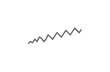
\begin{tikzpicture}[x=0.08em, y=0.08em, line width=0.4pt]
                \draw[FooterGray] (0,3) -- (1,4) -- (2,3.5) -- (3,5) -- (4,4) -- (5,6) -- (6,5.5) -- (7,4) -- (8,5) -- (9,7) -- (10,6) -- (11,5) -- (12,6.5) -- (13,8) -- (14,7) -- (15,6) -- (16,7.5) -- (17,9) -- (18,8) -- (19,7) -- (20,8.5) -- (21,10) -- (22,9) -- (23,8) -- (24,9.5);
            \end{tikzpicture}%
        }%
        \hskip0.5cm%
    }%
    \vskip6pt%
}

%=============================================================================
% PACKAGES
%=============================================================================
\usepackage[utf8]{inputenc}
\usepackage[T1]{fontenc}
\usepackage[english]{babel}
\usepackage{amsmath, amssymb, amsthm}
\usepackage{mathtools}
\usepackage{bm}
\usepackage{tikz}
\usetikzlibrary{arrows.meta, positioning, shapes, calc, decorations.pathreplacing, shadings}
\usepackage{booktabs}
\usepackage{multirow}
\usepackage{array}
\usepackage{graphicx}
\usepackage{hyperref}
\usepackage{colortbl}
\hypersetup{colorlinks=true, linkcolor=MainBlue, urlcolor=MainBlue}
\graphicspath{{../../logos/}{../../charts/}}
\hfuzz=2pt  % Suppress tiny overfull warnings (<2pt)
\vfuzz=2pt  % Suppress tiny vertical overfull warnings (<2pt)

%=============================================================================
% QUANTLET COMMAND
%=============================================================================
\newcommand{\quantlet}[2]{%
    \hfill\href{#2}{%
        \raisebox{-0.15em}{\includegraphics[height=0.7em]{ql_logo.png}}%
        \textcolor{MainBlue}{\tiny\ #1}%
    }%
}

%=============================================================================
% CENTRED MINIPAGE
%=============================================================================
\newenvironment{cminipage}[1]{%
    \par\noindent\hfill\begin{minipage}{#1}\ignorespaces
}{%
    \end{minipage}\hfill\null\par
}

%=============================================================================
% CUSTOM COMMANDS
%=============================================================================
\newcommand{\E}{\mathbb{E}}
\newcommand{\Var}{\text{Var}}
\newcommand{\Cov}{\text{Cov}}
\newcommand{\Corr}{\text{Corr}}
\newcommand{\R}{\mathbb{R}}
\newcommand{\RMSE}{\text{RMSE}}
\newcommand{\MAE}{\text{MAE}}
\newcommand{\MAPE}{\text{MAPE}}

\newcommand{\correct}{\textcolor{Forest}{\checkmark}}
\newcommand{\incorrect}{\textcolor{Crimson}{\texttimes}}

%=============================================================================
% TITLE INFORMATION
%=============================================================================
\title[Chapter 8: Seminar]{Chapter 8: Seminar --- Modern Extensions}
\subtitle{Bachelor program Faculty of Cybernetics, Statistics and Economic Informatics, Bucharest University of Economic Studies, Romania}
\author[Prof. dr. Daniel Traian Pele]{Prof. dr. Daniel Traian Pele\\[0.2cm]\footnotesize\texttt{danpele@ase.ro}}
\institute{Bucharest University of Economic Studies}
\date{Academic Year 2025--2026}

\begin{document}

%=============================================================================
% TITLE SLIDE
%=============================================================================
\begin{frame}[plain]
    \begin{tikzpicture}[remember picture, overlay]
        \fill[IDAred] (current page.north west) rectangle ([yshift=-0.15cm]current page.north east);
        \node[anchor=north west] at ([xshift=0.5cm, yshift=-0.3cm]current page.north west) {
            \href{https://www.ase.ro}{\includegraphics[height=1.1cm]{ase_logo.png}}
        };
        \node[anchor=north] at ([yshift=-0.3cm]current page.north) {
            \href{https://ai4efin.ase.ro}{\includegraphics[height=1.1cm]{ai4efin_logo.png}}
        };
        \node[anchor=north east] at ([xshift=-0.5cm, yshift=-0.3cm]current page.north east) {
            \href{https://www.digital-finance-msca.com}{\includegraphics[height=1.1cm]{msca_logo.png}}
        };
    \end{tikzpicture}
    \vfill
    \begin{center}
        {\Large\textcolor{MediumGray}{Time Series Analysis and Forecasting}}\\[0.3cm]
        {\Huge\textbf{\textcolor{MainBlue}{Chapter 8: Modern Extensions}}}\\[0.5cm]
        {\Large\textcolor{IDAred}{Seminar}}
    \end{center}
    \vfill

    \begin{tikzpicture}[remember picture, overlay]
        \fill[IDAred] (current page.south west) rectangle ([yshift=0.15cm]current page.south east);
        \node[anchor=south west] at ([xshift=0.5cm, yshift=0.8cm]current page.south west) {
            \href{https://theida.net}{\includegraphics[height=0.9cm]{ida_logo.png}}
        };
        \node[anchor=south] at ([xshift=-3cm, yshift=0.8cm]current page.south) {
            \href{https://blockchain-research-center.com}{\includegraphics[height=0.9cm]{brc_logo.png}}
        };
        \node[anchor=south] at ([yshift=0.8cm]current page.south) {
            \href{https://quantinar.com}{\includegraphics[height=0.9cm]{qr_logo.png}}
        };
        \node[anchor=south] at ([xshift=3cm, yshift=0.8cm]current page.south) {
            \href{https://quantlet.com}{\includegraphics[height=0.9cm]{ql_logo.png}}
        };
        \node[anchor=south east] at ([xshift=-0.5cm, yshift=0.8cm]current page.south east) {
            \href{https://ipe.ro/new}{\includegraphics[height=0.9cm]{acad_logo.png}}
        };
    \end{tikzpicture}
\end{frame}

%=============================================================================
% OUTLINE
%=============================================================================
\begin{frame}{Seminar Outline}
    \begin{cminipage}{0.95\textwidth}
    \textbf{\large Seminar structure:}

    \vspace{0.4cm}

    \begin{enumerate}
        \item[\textcolor{MainBlue}{\textbf{1.}}] \textbf{Review Quiz} -- Knowledge check
        \vspace{0.15cm}
        \item[\textcolor{MainBlue}{\textbf{2.}}] \textbf{True/False Questions} -- Conceptual checks
        \vspace{0.15cm}
        \item[\textcolor{MainBlue}{\textbf{3.}}] \textbf{Practice Problems} -- Applied practice
        \vspace{0.15cm}
        \item[\textcolor{MainBlue}{\textbf{4.}}] \textbf{Summary} -- Key takeaways
        \vspace{0.15cm}
        \item[\textcolor{MainBlue}{\textbf{5.}}] \textbf{AI-Assisted Exercises} -- Critical thinking
    \end{enumerate}
    \end{cminipage}
\end{frame}

%=============================================================================
% SECTION 1: REVIEW QUIZ
%=============================================================================
\section{Review Quiz}

\begin{frame}{Quiz 1: Hurst Exponent}
    \begin{alertblock}{Question}
        A time series has Hurst exponent $H = 0.8$. What does this indicate?
    \end{alertblock}

    \vspace{0.3cm}

    \begin{block}{Answer choices}
        \textcolor{MainBlue}{\textbf{(A)}} The series is a pure random walk\\[3pt]
        \textcolor{MainBlue}{\textbf{(B)}} The series has long memory and is persistent (trend-following)\\[3pt]
        \textcolor{MainBlue}{\textbf{(C)}} The series is anti-persistent (mean-reverting)\\[3pt]
        \textcolor{MainBlue}{\textbf{(D)}} The series is stationary I(0)
    \end{block}

    \vspace{0.5cm}
    \begin{flushright}\textit{Answer on next slide...}\end{flushright}
\end{frame}

\begin{frame}{Quiz 1: Answer}
    \begin{exampleblock}{Answer: B -- Long memory and persistence}
        \textbf{Hurst Exponent Interpretation:}
        \begin{itemize}
            \item $H = 0.5$: Random walk (no memory)
            \item $0.5 < H < 1$: \textbf{Persistence} -- trend continues
            \item $0 < H < 0.5$: Anti-persistence -- mean reversion
        \end{itemize}

        \vspace{0.3cm}
        With $H = 0.8 > 0.5$:
        \begin{itemize}
            \item The series has \textbf{long memory}
            \item Large values tend to be followed by large values
            \item Autocorrelations decay slowly (hyperbolically, not exponentially)
        \end{itemize}
    \end{exampleblock}
    \quantlet{TSA\_ch8\_hurst}{https://github.com/QuantLet/TSA/tree/main/TSA_ch8/TSA_ch8_hurst}
\end{frame}

\begin{frame}{Quiz 2: Fractional Differencing Parameter}
    \begin{alertblock}{Question}
        In the ARFIMA(p, d, q) model, the parameter $d$ can take values:
    \end{alertblock}

    \vspace{0.3cm}

    \begin{block}{Answer choices}
        \textcolor{MainBlue}{\textbf{(A)}} Only integer values (0, 1, 2, ...)\\[3pt]
        \textcolor{MainBlue}{\textbf{(B)}} Only $d = 0$ or $d = 1$\\[3pt]
        \textcolor{MainBlue}{\textbf{(C)}} Any real value, including fractional\\[3pt]
        \textcolor{MainBlue}{\textbf{(D)}} Only negative values
    \end{block}

    \vspace{0.5cm}
    \begin{flushright}\textit{Answer on next slide...}\end{flushright}
\end{frame}

\begin{frame}{Quiz 2: Answer}
    \begin{exampleblock}{Answer: C -- Any real value}
        \textbf{Fractional differencing}: $(1-L)^d$ with $d \in \mathbb{R}$

        \vspace{0.3cm}
        \textbf{Interpretation of $d$ values:}
        \begin{itemize}
            \item $d = 0$: Stationary series (ARMA)
            \item $0 < d < 0.5$: Long memory, stationary
            \item $d = 0.5$: Stationary/non-stationary boundary
            \item $0.5 < d < 1$: Long memory, non-stationary
            \item $d = 1$: Full differencing (classic ARIMA)
        \end{itemize}

        \vspace{0.2cm}
        \textbf{Relation to Hurst}: $d = H - 0.5$
    \end{exampleblock}
    \quantlet{TSA\_ch8\_arfima}{https://github.com/QuantLet/TSA/tree/main/TSA_ch8/TSA_ch8_arfima}
\end{frame}

\begin{frame}{Quiz 3: Long Memory in Financial Series}
    \begin{alertblock}{Question}
        In which financial series is long memory most commonly documented?
    \end{alertblock}

    \vspace{0.3cm}

    \begin{block}{Answer choices}
        \textcolor{MainBlue}{\textbf{(A)}} Stock prices\\[3pt]
        \textcolor{MainBlue}{\textbf{(B)}} Daily returns\\[3pt]
        \textcolor{MainBlue}{\textbf{(C)}} Volatility (squared returns)\\[3pt]
        \textcolor{MainBlue}{\textbf{(D)}} Trading volume
    \end{block}

    \vspace{0.5cm}
    \begin{flushright}\textit{Answer on next slide...}\end{flushright}
\end{frame}

\begin{frame}{Quiz 3: Answer}
    \begin{exampleblock}{Answer: C -- Volatility}
        \textbf{Stylized facts from finance:}
        \begin{itemize}
            \item \textbf{Returns}: Approximately memoryless ($H \approx 0.5$)
            \item \textbf{Volatility}: Pronounced long memory ($H \approx 0.7-0.9$)
        \end{itemize}

        \vspace{0.3cm}
        \textbf{Why?}
        \begin{itemize}
            \item Volatility clustering: turbulent periods followed by turbulent periods
            \item Persistence of shocks in variance
            \item FIGARCH: explicitly models long memory in volatility
        \end{itemize}

        \vspace{0.2cm}
        {\footnotesize This stylized fact is the basis for FIGARCH and HAR-RV models.}
    \end{exampleblock}
    \quantlet{TSA\_ch8\_long\_memory}{https://github.com/QuantLet/TSA/tree/main/TSA_ch8/TSA_ch8_long_memory}
\end{frame}

\begin{frame}{Quiz 4: Feature Engineering}
    \begin{alertblock}{Question}
        To apply Random Forest to time series, we must create:
    \end{alertblock}

    \vspace{0.3cm}

    \begin{block}{Answer choices}
        \textcolor{MainBlue}{\textbf{(A)}} Dummy variables for each observation\\[3pt]
        \textcolor{MainBlue}{\textbf{(B)}} Lag features and rolling statistics\\[3pt]
        \textcolor{MainBlue}{\textbf{(C)}} Fourier transforms of the series\\[3pt]
        \textcolor{MainBlue}{\textbf{(D)}} Only the first difference of the series
    \end{block}

    \vspace{0.5cm}
    \begin{flushright}\textit{Answer on next slide...}\end{flushright}
\end{frame}

\begin{frame}{Quiz 4: Answer}
    \begin{exampleblock}{Answer: B -- Lag features and rolling statistics}
        \textbf{Feature Engineering for Time Series:}

        \vspace{0.2cm}
        \begin{itemize}
            \item \textbf{Lag features}: $y_{t-1}, y_{t-2}, \ldots, y_{t-k}$
            \item \textbf{Rolling statistics}:
                \begin{itemize}
                    \item Rolling mean: $\bar{y}_{t,w}$
                    \item Rolling standard deviation: $\sigma_{t,w}$
                    \item Min/Max over window
                \end{itemize}
            \item \textbf{Calendar features}: day of week, month, etc.
        \end{itemize}

        \vspace{0.2cm}
        \textbf{Important}: Transforms the forecasting problem into a supervised regression problem!
    \end{exampleblock}
    \quantlet{TSA\_ch8\_ml\_forecast}{https://github.com/QuantLet/TSA/tree/main/TSA_ch8/TSA_ch8_ml_forecast}
\end{frame}

\begin{frame}{Quiz 5: Time Series Cross-Validation}
    \begin{alertblock}{Question}
        Why can't we use standard k-fold cross-validation for time series?
    \end{alertblock}

    \vspace{0.3cm}

    \begin{block}{Answer choices}
        \textcolor{MainBlue}{\textbf{(A)}} It's too slow for long series\\[3pt]
        \textcolor{MainBlue}{\textbf{(B)}} It violates temporal order and causes data leakage\\[3pt]
        \textcolor{MainBlue}{\textbf{(C)}} It only works for classification\\[3pt]
        \textcolor{MainBlue}{\textbf{(D)}} It requires too much data
    \end{block}

    \vspace{0.5cm}
    \begin{flushright}\textit{Answer on next slide...}\end{flushright}
\end{frame}

\begin{frame}{Quiz 5: Answer}
    \begin{exampleblock}{Answer: B -- Violates temporal order}
        \textbf{Problem with standard k-fold:}
        \begin{itemize}
            \item Shuffles observations temporally
            \item Trains on future data, tests on past
            \item \textbf{Data leakage} $\Rightarrow$ overestimated performance
        \end{itemize}

        \vspace{0.3cm}
        \textbf{Solution: Time Series Split (Walk-Forward)}
        \begin{center}
        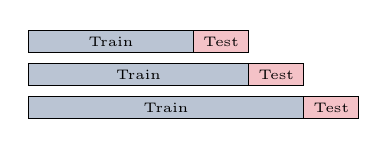
\begin{tikzpicture}[scale=0.7]
            \draw[fill=MainBlue!30] (0,0) rectangle (3,0.4) node[midway] {\tiny Train};
            \draw[fill=Crimson!30] (3,0) rectangle (4,0.4) node[midway] {\tiny Test};
            \draw[fill=MainBlue!30] (0,-0.6) rectangle (4,-0.2) node[midway] {\tiny Train};
            \draw[fill=Crimson!30] (4,-0.6) rectangle (5,-0.2) node[midway] {\tiny Test};
            \draw[fill=MainBlue!30] (0,-1.2) rectangle (5,-0.8) node[midway] {\tiny Train};
            \draw[fill=Crimson!30] (5,-1.2) rectangle (6,-0.8) node[midway] {\tiny Test};
        \end{tikzpicture}
        \end{center}
    \end{exampleblock}
    \quantlet{TSA\_ch8\_cross\_validation}{https://github.com/QuantLet/TSA/tree/main/TSA_ch8/TSA_ch8_cross_validation}
\end{frame}

\begin{frame}{Quiz 6: Feature Importance in Random Forest}
    \begin{alertblock}{Question}
        Feature importance in Random Forest for time series helps us:
    \end{alertblock}

    \vspace{0.3cm}

    \begin{block}{Answer choices}
        \textcolor{MainBlue}{\textbf{(A)}} Eliminate all low-importance variables\\[3pt]
        \textcolor{MainBlue}{\textbf{(B)}} Identify which lags and features are most predictive\\[3pt]
        \textcolor{MainBlue}{\textbf{(C)}} Determine Granger causality\\[3pt]
        \textcolor{MainBlue}{\textbf{(D)}} Calculate confidence intervals
    \end{block}

    \vspace{0.5cm}
    \begin{flushright}\textit{Answer on next slide...}\end{flushright}
\end{frame}

\begin{frame}{Quiz 6: Answer}
    \begin{exampleblock}{Answer: B -- Identifies predictive features}
        \textbf{Uses of feature importance:}
        \begin{itemize}
            \item Understanding temporal structure
            \item Selecting optimal number of lags
            \item Identifying relevant factors
        \end{itemize}

        \vspace{0.3cm}
        \textbf{Caution:}
        \begin{itemize}
            \item Importance does NOT imply causality
            \item Correlated variables may share importance
            \item Use for interpretation, not causal inference
        \end{itemize}
    \end{exampleblock}
    \quantlet{TSA\_ch8\_feature\_importance}{https://github.com/QuantLet/TSA/tree/main/TSA_ch8/TSA_ch8_feature_importance}
\end{frame}

\begin{frame}{Quiz 7: LSTM Advantage}
    \begin{alertblock}{Question}
        What is the main advantage of LSTM over simple RNNs?
    \end{alertblock}

    \vspace{0.3cm}

    \begin{block}{Answer choices}
        \textcolor{MainBlue}{\textbf{(A)}} It's faster to train\\[3pt]
        \textcolor{MainBlue}{\textbf{(B)}} It solves the vanishing/exploding gradient problem\\[3pt]
        \textcolor{MainBlue}{\textbf{(C)}} It requires less data\\[3pt]
        \textcolor{MainBlue}{\textbf{(D)}} It's easier to interpret
    \end{block}

    \vspace{0.5cm}
    \begin{flushright}\textit{Answer on next slide...}\end{flushright}
\end{frame}

\begin{frame}{Quiz 7: Answer}
    \begin{exampleblock}{Answer: B -- Solves the gradient problem}
        \textbf{Simple RNN Problem:}
        \begin{itemize}
            \item Gradients decay exponentially with sequence length
            \item Cannot learn long-term dependencies
        \end{itemize}

        \vspace{0.3cm}
        \textbf{LSTM Solution:}
        \begin{itemize}
            \item \textbf{Cell state}: Highway for information flow
            \item \textbf{Forget gate}: Decides what to forget
            \item \textbf{Input gate}: Decides what to remember
            \item \textbf{Output gate}: Decides what to output
        \end{itemize}

        \vspace{0.2cm}
        Gradients can ``flow'' through the cell state without degradation!
    \end{exampleblock}
    \quantlet{TSA\_ch8\_lstm}{https://github.com/QuantLet/TSA/tree/main/TSA_ch8/TSA_ch8_lstm}
\end{frame}

\begin{frame}{Quiz 8: Data Preparation for LSTM}
    \begin{alertblock}{Question}
        Before training an LSTM, data should be:
    \end{alertblock}

    \vspace{0.3cm}

    \begin{block}{Answer choices}
        \textcolor{MainBlue}{\textbf{(A)}} Log-transformed\\[3pt]
        \textcolor{MainBlue}{\textbf{(B)}} Normalized/scaled to [0,1] or [-1,1]\\[3pt]
        \textcolor{MainBlue}{\textbf{(C)}} Differenced twice\\[3pt]
        \textcolor{MainBlue}{\textbf{(D)}} Converted to integers
    \end{block}

    \vspace{0.5cm}
    \begin{flushright}\textit{Answer on next slide...}\end{flushright}
\end{frame}

\begin{frame}{Quiz 8: Answer}
    \begin{exampleblock}{Answer: B -- Normalized/scaled}
        \textbf{Why normalization?}
        \begin{itemize}
            \item Activation functions (sigmoid, tanh) work in limited ranges
            \item Faster convergence
            \item Numerical stability
        \end{itemize}

        \vspace{0.3cm}
        \textbf{Common methods:}
        \begin{itemize}
            \item \textbf{Min-Max}: $x' = \frac{x - x_{min}}{x_{max} - x_{min}}$ $\succ$ [0, 1]
            \item \textbf{Standard}: $x' = \frac{x - \mu}{\sigma}$ $\succ$ mean 0, std 1
        \end{itemize}

        \vspace{0.2cm}
        \textbf{Important}: Fit on train, transform on train+test!
    \end{exampleblock}
    \quantlet{TSA\_ch8\_lstm\_preprocessing}{https://github.com/QuantLet/TSA/tree/main/TSA_ch8/TSA_ch8_lstm_preprocessing}
\end{frame}

\begin{frame}{Quiz 9: LSTM Hyperparameters}
    \begin{alertblock}{Question}
        Which is NOT a typical LSTM hyperparameter?
    \end{alertblock}

    \vspace{0.3cm}

    \begin{block}{Answer choices}
        \textcolor{MainBlue}{\textbf{(A)}} Number of units (neurons) per layer\\[3pt]
        \textcolor{MainBlue}{\textbf{(B)}} Input sequence length\\[3pt]
        \textcolor{MainBlue}{\textbf{(C)}} Learning rate\\[3pt]
        \textcolor{MainBlue}{\textbf{(D)}} Differencing parameter $d$
    \end{block}

    \vspace{0.5cm}
    \begin{flushright}\textit{Answer on next slide...}\end{flushright}
\end{frame}

\begin{frame}{Quiz 9: Answer}
    \begin{exampleblock}{Answer: D -- The $d$ parameter}
        $d$ is specific to ARFIMA models, not LSTM!

        \vspace{0.3cm}
        \textbf{LSTM Hyperparameters:}
        \begin{itemize}
            \item \textbf{Architecture}: number of layers, units/layer
            \item \textbf{Sequence}: lookback length
            \item \textbf{Training}: learning rate, batch size, epochs
            \item \textbf{Regularization}: dropout, early stopping
        \end{itemize}

        \vspace{0.2cm}
        \textbf{Tuning}: Grid search or Bayesian optimization with time series CV
    \end{exampleblock}
    \quantlet{TSA\_ch8\_lstm\_tuning}{https://github.com/QuantLet/TSA/tree/main/TSA_ch8/TSA_ch8_lstm_tuning}
\end{frame}

%=============================================================================
% TRUE/FALSE QUESTIONS
%=============================================================================
\section{True/False Questions}

\begin{frame}{True or False? --- Questions}
    \begin{cminipage}{0.95\textwidth}
    \footnotesize
    \begin{center}
    \begin{tabular}{p{9cm}c}
        \toprule
        \textbf{Statement} & \textbf{T/F?} \\
        \midrule
        1. ARFIMA models can capture long-term dependence. & ? \\[0.15cm]
        2. The parameter $d$ in ARFIMA must be an integer. & ? \\[0.15cm]
        3. LSTM networks are better than ARIMA in all situations. & ? \\[0.15cm]
        4. Random Forest requires manually created features. & ? \\[0.15cm]
        5. Standard cross-validation (k-fold) is suitable for time series. & ? \\[0.15cm]
        6. The Hurst exponent $H > 0.5$ indicates positive long memory. & ? \\
        \bottomrule
    \end{tabular}
    \end{center}
    \end{cminipage}
\end{frame}

\begin{frame}{True or False? --- Answers}
    \begin{cminipage}{0.95\textwidth}
    \scriptsize
    \begin{center}
    \begin{tabular}{p{7.5cm}cc}
        \toprule
        \textbf{Statement} & \textbf{T/F} & \textbf{Explanation} \\
        \midrule
        1. ARFIMA captures long-term dependence. & \textcolor{Forest}{\textbf{T}} & {\tiny Fractional $d$} \\[0.08cm]
        2. $d$ in ARFIMA must be an integer. & \textcolor{Crimson}{\textbf{F}} & {\tiny $d \in (0, 0.5)$ fractional} \\[0.08cm]
        3. LSTM better than ARIMA always. & \textcolor{Crimson}{\textbf{F}} & {\tiny Depends on data and sample} \\[0.08cm]
        4. RF requires manual features. & \textcolor{Forest}{\textbf{T}} & {\tiny Lags, calendar, etc.} \\[0.08cm]
        5. k-fold CV suitable for time series. & \textcolor{Crimson}{\textbf{F}} & {\tiny Violates temporal ordering} \\[0.08cm]
        6. $H > 0.5$ indicates positive long memory. & \textcolor{Forest}{\textbf{T}} & {\tiny $H = 0.5$: no memory} \\
        \bottomrule
    \end{tabular}
    \end{center}
    \end{cminipage}
\end{frame}

%=============================================================================
% SECTION 4: PRACTICAL PROBLEMS
%=============================================================================
\section{Practice Problems}

\begin{frame}{Problem 1: Hurst Exponent Estimation}
    \begin{block}{Exercise}
        Given daily Bitcoin returns, estimate the Hurst exponent using the R/S method and interpret the result.
    \end{block}

    \vspace{0.3cm}
    \textbf{Solution Steps:}
    \begin{enumerate}
        \item Calculate mean over subintervals of different lengths $n$
        \item For each $n$: calculate Range($R$) and Std($S$)
        \item The ratio $R/S$ grows as $n^H$
        \item Fit regression: $\log(R/S) = H \cdot \log(n) + c$
    \end{enumerate}

    \vspace{0.2cm}
    \textbf{Python code}: \texttt{nolds.hurst\_rs(returns)}
\end{frame}

\begin{frame}{Problem 1: Solution and Interpretation}
    \begin{exampleblock}{Typical Bitcoin Results}
        \begin{itemize}
            \item Returns: $H \approx 0.45-0.55$ (approximately random walk)
            \item Volatility (|returns|): $H \approx 0.75-0.85$ (long memory!)
        \end{itemize}
    \end{exampleblock}

    \vspace{0.3cm}
    \textbf{Interpretation:}
    \begin{itemize}
        \item Returns are hard to predict (EMH approximately valid)
        \item Volatility is predictable over long horizons
        \item Implications for risk management and VaR
    \end{itemize}

    \vspace{0.2cm}
    \textbf{Application}: FIGARCH models may outperform standard GARCH
    \quantlet{TSA\_ch8\_hurst}{https://github.com/QuantLet/TSA/tree/main/TSA_ch8/TSA_ch8_hurst}
\end{frame}

\begin{frame}{Problem 2: Random Forest for Forecasting}
    \begin{block}{Exercise}
        Build a Random Forest model for 1-day ahead Bitcoin price forecasting. Evaluate using TimeSeriesSplit.
    \end{block}

    \vspace{0.3cm}
    \textbf{Pipeline:}
    \begin{enumerate}
        \item \textbf{Feature engineering}:
            \begin{itemize}
                \item Lags: $y_{t-1}, y_{t-2}, \ldots, y_{t-7}$
                \item Rolling mean/std: 7, 14, 30 days
            \end{itemize}
        \item \textbf{Train/Test split}: TimeSeriesSplit(n\_splits=5)
        \item \textbf{Model}: RandomForestRegressor(n\_estimators=100)
        \item \textbf{Evaluation}: RMSE, MAE, Direction Accuracy
    \end{enumerate}
\end{frame}

\begin{frame}{Problem 2: Code and Results}
    \begin{exampleblock}{Python Code}
        {\footnotesize
        \texttt{from sklearn.ensemble import RandomForestRegressor}\\
        \texttt{from sklearn.model\_selection import TimeSeriesSplit}\\[0.2cm]
        \texttt{tscv = TimeSeriesSplit(n\_splits=5)}\\
        \texttt{rf = RandomForestRegressor(n\_estimators=100)}\\[0.2cm]
        \texttt{for train\_idx, test\_idx in tscv.split(X):}\\
        \texttt{~~~~rf.fit(X[train\_idx], y[train\_idx])}\\
        \texttt{~~~~pred = rf.predict(X[test\_idx])}
        }
    \end{exampleblock}

    \vspace{0.2cm}
    \textbf{Typical results}:
    \begin{itemize}
        \item Direction accuracy: 52-55\% (slightly above random)
        \item Feature importance: lag-1 and rolling\_std dominate
    \end{itemize}
    \quantlet{TSA\_ch8\_random\_forest}{https://github.com/QuantLet/TSA/tree/main/TSA_ch8/TSA_ch8_random_forest}
\end{frame}

\begin{frame}{Problem 3: LSTM for Time Series}
    \begin{block}{Exercise}
        Implement a simple LSTM model for Bitcoin forecasting. Compare with Random Forest.
    \end{block}

    \vspace{0.3cm}
    \textbf{Simple LSTM Architecture:}
    \begin{enumerate}
        \item Input: 30-day sequences
        \item LSTM layer: 50 units
        \item Dense output: 1 neuron (forecast)
        \item Loss: MSE, Optimizer: Adam
    \end{enumerate}

    \vspace{0.2cm}
    \textbf{Important steps}:
    \begin{itemize}
        \item MinMaxScaler normalization
        \item Reshape to [samples, timesteps, features]
        \item Early stopping to prevent overfitting
    \end{itemize}
\end{frame}

\begin{frame}{Problem 3: LSTM Code}
    \begin{exampleblock}{Keras/TensorFlow Code}
        {\footnotesize
        \texttt{from tensorflow.keras.models import Sequential}\\
        \texttt{from tensorflow.keras.layers import LSTM, Dense}\\[0.2cm]
        \texttt{model = Sequential([}\\
        \texttt{~~~~LSTM(50, input\_shape=(30, 1)),}\\
        \texttt{~~~~Dense(1)}\\
        \texttt{])}\\[0.2cm]
        \texttt{model.compile(optimizer='adam', loss='mse')}\\
        \texttt{model.fit(X\_train, y\_train, epochs=50,}\\
        \texttt{~~~~~~~~~~validation\_split=0.1, verbose=0)}
        }
    \end{exampleblock}

    \vspace{0.2cm}
    \textbf{Typical RF vs LSTM comparison}:
    \begin{itemize}
        \item RMSE similar (LSTM slightly better on smooth data)
        \item RF: faster, more interpretable
        \item LSTM: captures complex patterns better
    \end{itemize}
    \quantlet{TSA\_ch8\_lstm}{https://github.com/QuantLet/TSA/tree/main/TSA_ch8/TSA_ch8_lstm}
\end{frame}

%=============================================================================
% SECTION 5: SUMMARY
%=============================================================================
\section{Summary}

\begin{frame}{Summary: When to Use Each Method}
    \vspace{-0.9cm}
    \begin{block}{ARFIMA}
        \begin{itemize}
            \item Series with long memory (volatility, hydrology)
            \item When $0 < d < 0.5$ is theoretically justified
            \item Statistical interpretability is important
        \end{itemize}
    \end{block}

    \begin{block}{Random Forest}
        \begin{itemize}
            \item Nonlinear relationships between features
            \item Feature importance for understanding
            \item Structured data, not too long series
        \end{itemize}
    \end{block}

    \begin{block}{LSTM}
        \begin{itemize}
            \item Long sequences with complex dependencies
            \item Sufficient data for deep learning
            \item Patterns difficult to capture with classical methods
        \end{itemize}
    \end{block}
\end{frame}

\begin{frame}[shrink=5]{Key Formulas}
    \vspace{-0.8cm}
    \begin{block}{ARFIMA and Long Memory}
        \begin{itemize}
            \item Fractional differencing: $(1-L)^d y_t = \varepsilon_t$
            \item Hurst exponent: $d = H - 0.5$
            \item ACF for long memory: $\rho(k) \sim k^{2d-1}$ (slow decay)
        \end{itemize}
    \end{block}

    \begin{block}{Machine Learning}
        \begin{itemize}
            \item Lag feature: $X_t = [y_{t-1}, y_{t-2}, \ldots, y_{t-k}]$
            \item RMSE: $\sqrt{\frac{1}{n}\sum(y_i - \hat{y}_i)^2}$
            \item Direction Accuracy: $\frac{1}{n}\sum \mathbf{1}[\text{sign}(\Delta y) = \text{sign}(\Delta \hat{y})]$
        \end{itemize}
    \end{block}

    \begin{block}{LSTM}
        \begin{itemize}
            \item Forget gate: $f_t = \sigma(W_f \cdot [h_{t-1}, x_t] + b_f)$
            \item Cell update: $C_t = f_t * C_{t-1} + i_t * \tilde{C}_t$
        \end{itemize}
    \end{block}
\end{frame}

%=============================================================================
% AI-ASSISTED EXERCISES
%=============================================================================
\section{AI-Assisted Exercises}

\begin{frame}{AI Exercise: Critical Thinking}
    \vspace{-0.3cm}
    \begin{cminipage}{0.95\textwidth}
    \begin{block}{Test this prompt in ChatGPT/Claude/Copilot}
        \textit{``Download hourly electricity consumption data. Compare three approaches: (1) ARIMA, (2) Random Forest with lag features, (3) LSTM. Use time series cross-validation, report RMSE and directional accuracy for each.''}
    \end{block}
    \vspace{-2mm}
    {\footnotesize
    \begin{enumerate}\setlength{\itemsep}{0pt}
        \item Did the AI use proper time series cross-validation (no future data leakage)?
        \item Are the lag features for Random Forest correctly constructed?
        \item Is the LSTM data properly scaled and sequenced?
        \item Does the comparison use the same test set for all three models?
        \item Which model performs best and why? Is this consistent with theory?
    \end{enumerate}
    }
    \vspace{-2mm}
    \begin{alertblock}{}
        {\footnotesize \textbf{Warning}: AI-generated code may run without errors and look professional. That does not mean it is correct.}
    \end{alertblock}
    \end{cminipage}
\end{frame}

%=============================================================================
% THANK YOU SLIDE
%=============================================================================
\begin{frame}{}
    \begin{cminipage}{0.95\textwidth}
    \centering
    \Huge\textcolor{IDAred}{Thank You!}

    \vspace{1cm}

    \Large\textcolor{MainBlue}{Questions?}

    \vspace{0.8cm}

    \normalsize
    Seminar materials are available at: \url{https://danpele.github.io/Time-Series-Analysis/}

    \vspace{0.2cm}

    \href{https://quantlet.com}{\raisebox{-0.15em}{\includegraphics[height=0.8em]{ql_logo.png}} Quantlet} \hspace{0.5cm}
    \href{https://quantinar.com}{\raisebox{-0.15em}{\includegraphics[height=0.8em]{qr_logo.png}} Quantinar}
    \end{cminipage}
\end{frame}

%=============================================================================
% BIBLIOGRAPHY
%=============================================================================
\begin{frame}{Bibliography I}
    \begin{block}{Fundamental Textbooks}
        {\small
        \begin{itemize}
            \item Hyndman, R.J., \& Athanasopoulos, G. (2021). \textit{Forecasting: Principles and Practice}, 3rd ed., OTexts.
            \item Shumway, R.H., \& Stoffer, D.S. (2017). \textit{Time Series Analysis and Its Applications}, 4th ed., Springer.
            \item Brockwell, P.J., \& Davis, R.A. (2016). \textit{Introduction to Time Series and Forecasting}, 3rd ed., Springer.
        \end{itemize}
        }
    \end{block}

    \begin{exampleblock}{Financial Time Series}
        {\small
        \begin{itemize}
            \item Tsay, R.S. (2010). \textit{Analysis of Financial Time Series}, 3rd ed., Wiley.
            \item Franke, J., H\"ardle, W.K., \& Hafner, C.M. (2019). \textit{Statistics of Financial Markets}, 4th ed., Springer.
        \end{itemize}
        }
    \end{exampleblock}
\end{frame}

\begin{frame}{Bibliography II}
    \begin{block}{Modern Approaches and Machine Learning}
        {\small
        \begin{itemize}
            \item Nielsen, A. (2019). \textit{Practical Time Series Analysis}, O'Reilly Media.
            \item Petropoulos, F., et al. (2022). \textit{Forecasting: Theory and Practice}, International Journal of Forecasting.
            \item Makridakis, S., Spiliotis, E., \& Assimakopoulos, V. (2020). The M4 Competition, International Journal of Forecasting.
        \end{itemize}
        }
    \end{block}

    \begin{exampleblock}{Online Resources and Code}
        {\small
        \begin{itemize}
            \item \textbf{Quantlet}: \url{https://quantlet.com} --- Code repository for statistics
            \item \textbf{Quantinar}: \url{https://quantinar.com} --- Quantitative methods learning platform
            \item \textbf{GitHub TSA}: \url{https://github.com/QuantLet/TSA} --- Python code for this seminar
        \end{itemize}
        }
    \end{exampleblock}
\end{frame}

\end{document}
